\chapter{Implémentation} \label{ch:implementation}

Le modèle se construit sur différents niveaux d’abstractions. L'exécution d'une simulation s'effectue en plusieurs étapes, du plus général au plus détaillé.

\section{Main}

Le main est la structure du plus haut niveau du modèle est sert d'interface pour l'utilisateur. A ce niveau, il est possible d'instancier plusieurs simulations avec des paramètres choisis. Afin de pouvoir exécuter une simulation il est nécessaire d'y ajouter un fichier de configuration contenant les paramètres de la simulation ainsi que de lui fournir un générateur de nombres aléatoires.\\

Par conséquent, chaque simulation demande deux arguments pour se lancer. Le premier est un chemin vers un dossier dans lequel se trouve le fichier de configuration. Le deuxième argument est générateur pseudo-aléatoire permettant la génération de nombres aléatoires indispensables à la simulation.\\ 

Le chemin vers le dossier est la racine de la simulation. Dans ce dossier racine doit se trouver le fichier de configuration. Le fichier de configuration doit avoir le nom suivant : **config.txt**.  A la fin de la simulation, le programme écrit les résultats dans un sous-dossier à la racine. Ces résultats sont des fichiers CSV contenant des informations sur la simulation.\\

L'avantage de dédier un générateur pseudo-aléatoire à chaque simulation est de permettre de ré-exécuter les simulations en obtenant toujours les mêmes résultats, ce qui confère à l'algorithme la propriété d'idempotence.\\

Un ficher de configuration est un ficher texte contenant des lignes formées de mots clefs accompagnée de leur valeur. Un analyseur syntaxique parse le fichier puis les tokens sont analysés par un analyseur lexical qui s'occupe d'assigner les variables du modèles avec les valeurs lues dans le fichier de configuration.\\ 

La syntaxe du fichier de configuration doit être respectée. Les valeurs peuvent être modifiées par contre les noms doivent être identiques. L'analyseur lexicale n'est pas sensible aux espaces insérés entre les noms, le "=" ainsi que les valeurs.

\begin{minted}
[
frame=lines,
framesep=2mm,
baselinestretch=1.2,
bgcolor=LightGray,
fontsize=\footnotesize,
linenos
]
{c++}

TAILLE_SYSTEME = 894
NOMBRE_INDIVIDUS = 100000
ITERATIONS = 150
RERUN_LIMIT = 1000
FAIL_SEUIL = 10
GENOME_INIT_I = 0
GENOME_DIVERSITY_I = 0
GENOME_INIT_AP = 0
VITESSE_MUTATIONS_AP = 0
CHARGE_VIRALE = 1
PARAMETRE_FONCTION = 1
CELLULE_AP = 0
SURVIE_AP = 0
NOMBRE_MOUVEMENT = 1
PERFECT_MIX = false
TEMPS_AVANT_IMMUNITE = 1
IMMUNITE_MECANISME = false
RESISTANCE_MECANISME = false
\end{minted}

Voici la structure d'un fichier de configuration. Chaque ligne est composée d'un paramètre avec une valeur associée. 

\section{Initialisation}

La phase d'initialisation prépare le système pour une simulation. La première étape est de lire le fichier de configuration et d'assigner les valeurs lues aux variables de la simulation. Ensuite il faut allouer de la mémoire pour tous les objets du système. Un objet du système est un acteur donc il s'agit soit d'un individu, soit d'un pathogène. Le nombre d'individus du système est déterminé par le paramètre "NOMBRE\_INDIVIDUS" et une liste de pointeurs sur ces individus est créée. Cette liste est de taille fixe et contient tous les individus du système. Contrairement aux individus, les agents pathogènes ne sont pas contenus dans une liste fixe à cause de leur nombre pouvant changer. En effet, un agent pathogène est un objet à part entière si et seulement si il contamine une cellule. Nous utilisons donc une liste doublement chaînée pour stocker ces objets. Cette structure permet de supprimer un élément au milieu de la liste sans créer de trou.\\ 

Le paramètre "TAILLE\_SYSTEME" nous indique la taille de la grille. La grille allouée est une matrice de pointeurs pouvant pointer sur les acteurs qui sont les objets du système. \\

\begin{figure}[h]
\centering
\captionsetup{justification=centering}
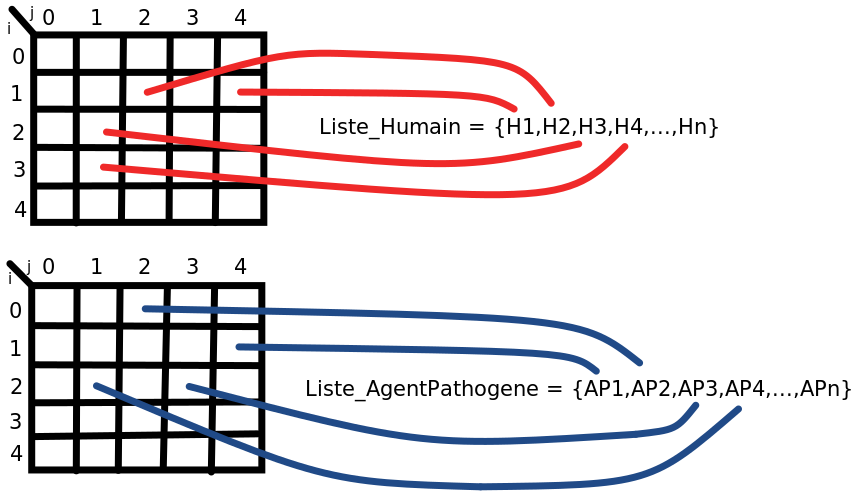
\includegraphics[scale=0.4]{Images/MatricesPointeurs.png}
\caption[Matrices de pointeurs]{L'espace est représenté par deux matrices de pointeurs de la taille du système. Chacune de ces matrices pointe exclusivement sur un type d'acteurs.}
\end{figure}

Après avoir créé les structures de données il faut générer les génomes des individus. Le génome initial de référence est donnée par le paramètre "GENOME\_INIT\_I". Ce dernier sert de base pour la génération des génomes des individus. Le paramètre "GENOME\_DIVERSITY\_I" détermine le niveau de déviation par rapport aux génome de référence. Par conséquent, pour attribuer des génomes aux individus on part du génome de référence et modifions aléatoirement un nombre de bits déterminé par le paramètre "GENOME\_DIVERSITY\_I". Par exemple, avec GENOME\_DIVERSITY\_I = 1, tous les individus auront le génome de référence avec un bits choisi aléatoirement dans la séquence qui sera modifié. Ce mécanisme permet d'obtenir des génomes avec un certain degré de proximité à une certaine valeur choisie. Le modèle n'intègre pas de mécanise pour générer des génomes pour les agents pathogènes car la simulation ne commence qu'avec un seul agent pathogène qui porte le génome défini par "GENOME\_INIT\_AP".\\

L'étape suivante est de disposer tous les individus sur la grille et ceci aléatoirement. Finalement il faut contaminer un premier individu avec la premier pathogène défini par le paramètre "GENOME\_INIT\_AP". 

\section{Exécution de la simulation}

Une grande partie des calculs de la simulation se font à cette étape. Cette phase s'effectue un nombre de fois équivalent à la valeur du paramètre "ITERATIONS". Chaque itération sert à actualiser, à un moment donné le système en entier. La première partie de cette étape est la prise de mesures et l'écriture des mesures dans les fichier CSV. Les données récoltées sont le nombre de contaminés, le nombre d'agents pathogènes différents ainsi que le nombre d'individus ayant au moins une immunité. Toutes les mesures du systèmes qui doivent s'effectuer à chaque itération se font à cette étape. Faire des mesures au fur et à mesure de la simulation nous évite de devoir sauvegarder toutes les données.\\

La prochaine étape est la construction d'une permutation des indices de la liste contenant les individus. Pour que le système soit aléatoire il est important de ne pas actualiser tous les individus dans le même ordre à chaque itération. C'est la raison pour laquelle nous permutons les indices de la liste des individus à chaque itération et la parcourons en suivant les indices permutés. Ceci permet d'actualiser tous les individus du système dans un ordre aléatoire.\\

Vient ensuite les phases de mise à jour et actions des acteurs du système. Le type d'acteur le plus simple est les agents pathogènes contaminant des cellules. Ces derniers sont détachés des individus et sont donc des objets à part entière. L'actualisation de ces agents pathogène s'effectue en une seule étape. Nous parcourons tous les agents pathogènes contaminant des cellules (l'ordre ici n'est pas important) et déterminons si les pathogènes survivent à cette itération. La probabilité de survie d'un tel agent pathogène est déterminé par le paramètre "SURVIE\_AP". Ce facteur donne la probabilité qu'un agent pathogène contaminant une cellule survive à cette itération.\\

Finalement, la dernière étape de la phase est l'actualisation de tous les individus du système. Cette étape est de loin la plus coûteuse en temps. En premier il s'agit de parcourir un à un tous les individus en respectant les indices permutés. L'actualisation d'un individu se fait en deux étapes. La première étape consiste à calculer les interactions et mettre à jour son état interne. La seconde est d'effectuer un déplacement.\\ 

La première chose à faire lorsque nous souhaitons actualiser un individu est de regarder si cet individu est contaminé. Si l'individu est déjà contaminé il est inutile de calculer les interactions avec ses voisins étant donnée qu'il est hôte d'un pathogène. Il nous reste donc à actualiser son état interne. Dans cette situation, notre individu n'a que trois issues. La première est d'être naturellement résistant au pathogène. La seconde est de l'immuniser au pathogène et la troisième est de conserver le pathogène. La distinction entre résistance naturelle et immunisation n'est qu'une question de temps. Il s'agit en réalité exactement du même mécanisme mais à partir d'un certain temps en étant contaminé, nous déterminons que l'individu s'immunise. Chaque individu compte le nombre d'itération depuis lequel il est contaminé. Si l'individu à une certaine itération se débarrasse du pathogène, le compteur déterminera si il s'agit d'une immunité ou d'une résistance naturelle.\\

Le paramètre booléen "IMMUNITE\_MECANISME" du modèle détermine si le mécanisme d'immunisation est actif ou non. Il en est de même pour le paramètre booléen "RESISTANCE\_MECANISME". Désactiver ces mécaniques permet de simuler des systèmes ou l'immunisation est impossible pour quelques raisons. Il est aussi possible de déterminer le seuil temporelle différenciant la résistance naturelle de l'immunisation avec le paramètre "TEMPS\_AVANT\_IMMUNITE". C'est-à-dire que cette variable détermine le temps minimal nécessaire pour que le rejet du pathogène soit considéré comme immunité.\\

Pour déterminer si un hôte contaminé rejette ou non son agent pathogène à une certaine itération, nous utilisons une fonction calculant la compatibilité entre le pathogène et l'individu. La première étape pour calculer la compatibilité entre deux organismes est d'évaluer la distance de Hamming entre les deux séquences de génomes. L'entier résultant doit ensuite être converti en probabilité car l'individu a une certaine probabilité de se débarrasser du pathogène à cette itération. La conversion s'effectue par une fonction dont une variable est définie par le paramètre du modèle "PARAMETRE\_FONCTION".\\
$$
f(d) = \frac{d^{PARAMETRE\_FONCTION}}{32^{PARAMETRE\_FONCTION}} = (\frac{d}{32})^{PARAMETRE\_FONCTION}
$$
Le paramètre $d$ est la distance de Hamming entre les deux génomes des acteurs. Cette fonction traduit la distance de Hamming en une probabilité car $d$ ne peut varier que entre $[0,32]$.

\begin{figure}[h]
  \centering
    \captionsetup{justification=centering}
  \begin{minipage}[b]{0.4\textwidth}
    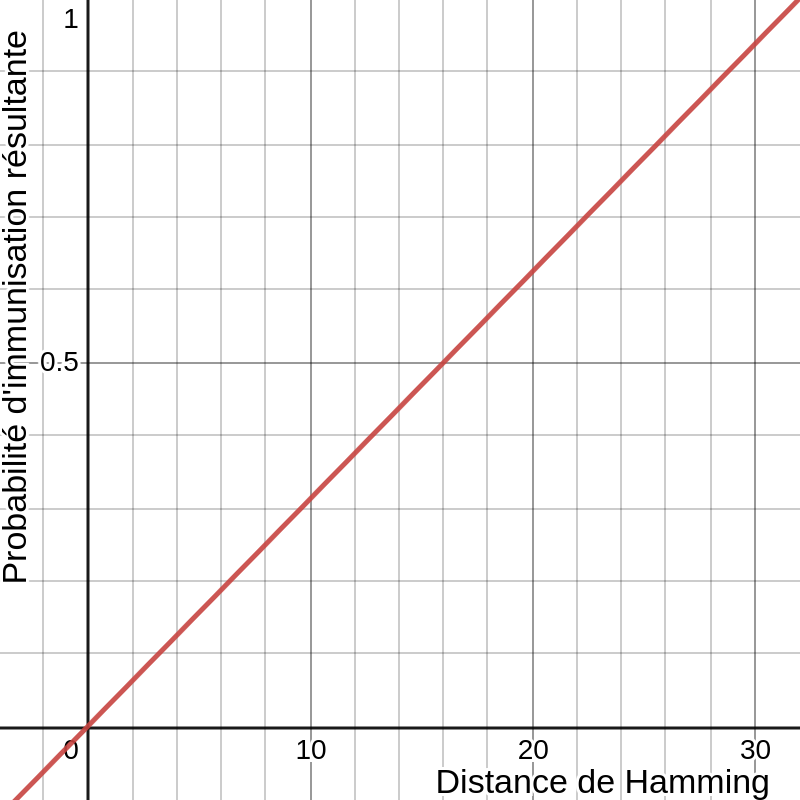
\includegraphics[width=\textwidth]{Images/fonction_1.png}
    \caption[Fonction de converstion en probabilité (facteur 4)]{Fonction de conversion de la distance de Hamming en probabilité avec $PARAMETRE\_FONCTION = 1$}
  \end{minipage}
  \hfill
  \begin{minipage}[b]{0.4\textwidth}
    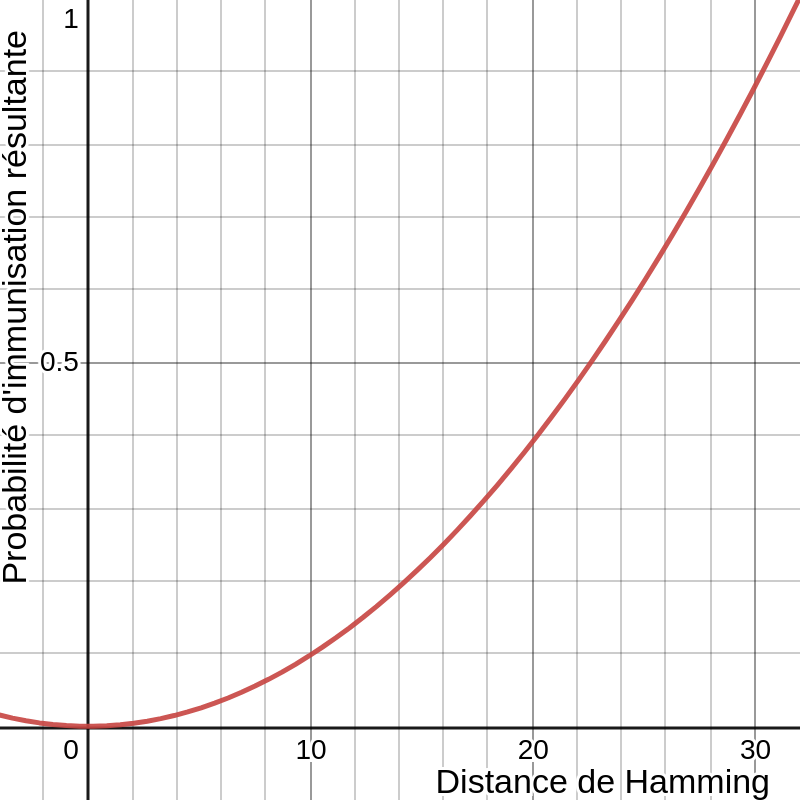
\includegraphics[width=\textwidth]{Images/fonction_2.png}
    \caption[Fonction de converstion en probabilité (facteur 4)]{Fonction de conversion de la distance de Hamming en probabilité avec $PARAMETRE\_FONCTION = 2$}
  \end{minipage}
\end{figure}

\begin{figure}[h]
  \centering
    \captionsetup{justification=centering}
  \begin{minipage}[b]{0.4\textwidth}
    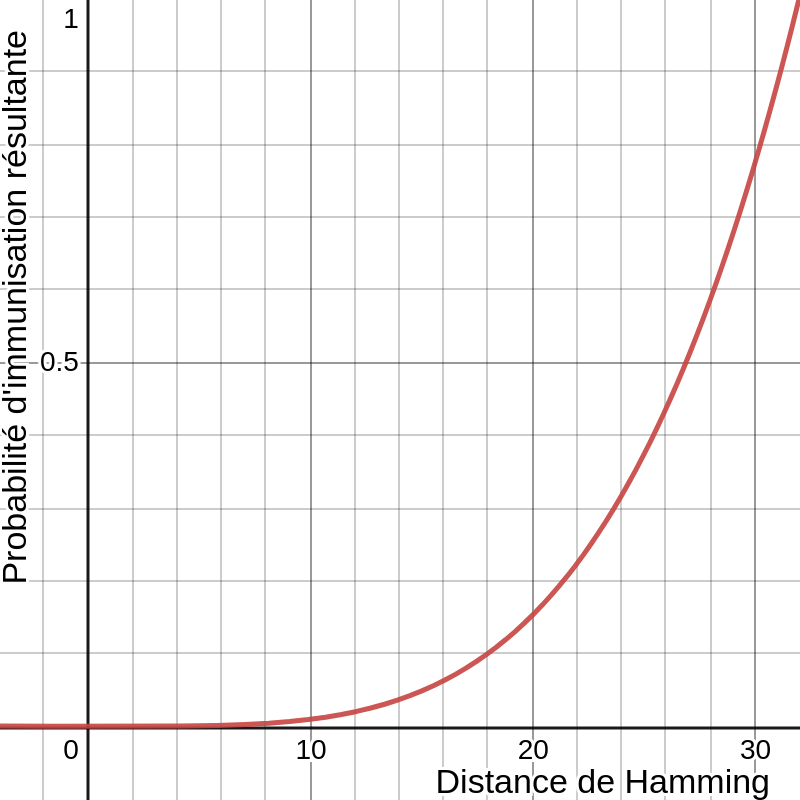
\includegraphics[width=\textwidth]{Images/fonction_4.png}
    \caption[Fonction de converstion en probabilité (facteur 4)]{Fonction de conversion de la distance de Hamming en probabilité avec $PARAMETRE\_FONCTION = 4$}
  \end{minipage}
  \hfill
  \begin{minipage}[b]{0.4\textwidth}
    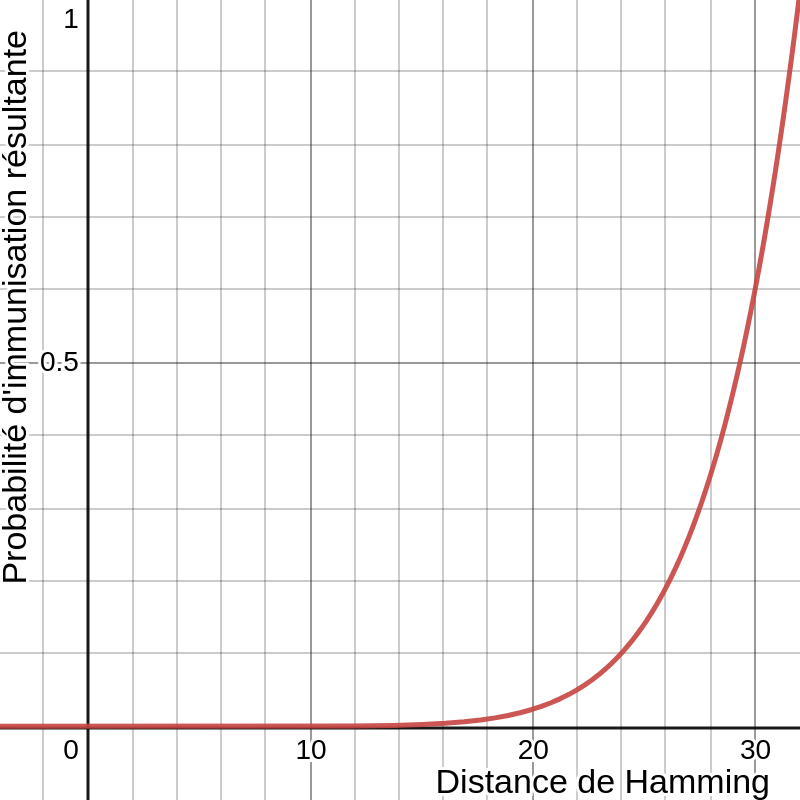
\includegraphics[width=\textwidth]{Images/fonction_8.png}
    \caption[Fonction de converstion en probabilité (facteur 4)]{Fonction de conversion de la distance de Hamming en probabilité avec $PARAMETRE\_FONCTION = 8$}
  \end{minipage}
\end{figure}

Par conséquent les images de notre formules sont bornées entre $[0,1]$. Le paramètre de fonction permet de modifier l'allure de la courbe sans modifier les bornes. Une petite valeur "PARAMETRE\_FONCTION" traduit de grandes probabilités d'immuniser l'individu et inversement une grande valeur du paramètre traduit en de faibles probabilités d'immunisation.\\

Lorsqu'un individu est décrété naturellement résistant à un pathogène, il se contente uniquement de s'en débarrasser. Par contre si l'individu s'immunise au pathogène, le génome de ce dernier est enregistré dans les attributs de l'individu.\\ 

Comme expliqué ci-dessus, à chaque itération, chaque individu contaminé a une chance de se débarrasser de son pathogène. Si l'hôte contaminé n'y parvient pas, alors le pathogène a la possibilité de muter. Le facteur de mutation de la simulation est donné par le paramètre "VITESSE\_MUTATIONS\_AP". Ce paramètre borné borné entre $[0,1]$ détermine la probabilité qu'a un pathogène de muter dans un individu. En cas de mutation, un agent pathogène complémente aléatoirement un seul bit de sa séquence de génome.\\

Le processus de mise à jour pour les individus non contaminés est bien différent. Ces derniers n'intègrent pas de pathogène par conséquent nous nous intéressons aux interactions avec les autres acteurs. Un individu sain est soumis à deux types d'interactions, la première est l'interaction avec des agents pathogènes contaminant des cellules de la grille et la seconde est l’interaction avec des individus dans le voisinage.\\

Les deux types d'interactions suivent la même méthodologie. La première étape de toutes interactions est donné par le paramètre "CHARGE\_VIRALE". Le paramètre borné entre $[0,1]$ détermine la probabilité qu'une interaction se produise entre deux acteurs en contact. La deuxième étape est la vérification des immunités. En effet, si l'individu est déjà immunisé au pathogène le contaminant, rien ne se produit. Sans protection l'individu devient contaminé par le pathogène.\\

L'actualisation d'un individu se termine par une série de mouvements dans l'espace. A chaque itération un individu peut se déplacer un nombre de fois égal au paramètre "NOMBRE\_MOUVEMENT". Par conséquent un individu peut se déplacer de une cellule le nombre de fois décrit par le paramètre. Le choix de la direction du déplacement est déterminé avant la vérification des cellules disponibles. En cas d'échec de déplacement dû à la non disponibilité de la cellule destination, le mouvement non effectué est tout de même comptabilisé. Cela signifie que si le paramètre de mouvement est défini à $10$, les individus se déplacent à chaque itération d'un nombre de cellules variant entre $[0,10]$ en fonction de la disponibilité.\\

Un individu contaminé se déplaçant a une chance de contaminer l'espace qu'il quitte. La probabilité de réaliser cet événement est donnée par le paramètre "CELLULE\_AP" borné de $[0,1]$. En cas de contamination de cellule un nouvel objet agent pathogène est créé et porte le génome du pathogène de l'individu contaminé. 

\section{Prise des mesures}

La phase des mesures s'effectue après le déroulement de la simulation. Toutes les mesures nécessitant que la simulation ait abouti s'exécutent dans cette section. Comme vu dans la partie précédente, certaines mesures doivent s'effectuer au fil de la simulation.\\ 

La seule mesure du modèle de cette catégorie est le calcul du nombre de fois que les individus ont été contaminés. Chaque individu du système compte le nombre de fois ou il a été contaminé par des agents pathogènes différents. Est compté comme contamination tout cycle débutant par la contraction du pathogène jusqu'à l'immunisation à ce dernier. 

\section{Fermeture}

La phase de fermeture de la simulation effectue deux actions. La première est de fermer tous les fichier CSV et la seconde est de libérer tous les espaces mémoires alloués par la simulation.